\documentclass[10pt]{article}
\usepackage[utf8]{inputenc}
\usepackage{url}
\usepackage{hyperref}
\usepackage{amsmath}
\usepackage{amsfonts}
\usepackage{amssymb}
\usepackage{graphicx}
\graphicspath{ {./images/} }
\usepackage{float}
\usepackage{lipsum}
\usepackage{sectsty}
\sectionfont{\centering}
\usepackage{multicol}
\usepackage{xcolor}
\usepackage{textcomp}
\usepackage{natbib}
\usepackage{graphicx}
\usepackage{listings}
\usepackage{xcolor}
\usepackage[font=small]{caption}
\addtolength{\abovecaptionskip}{-3mm}
\addtolength{\textfloatsep}{-5mm}
\setlength\columnsep{20pt}

\usepackage[a4paper,left=1.50cm, right=1.50cm, top=2cm, bottom=3cm]{geometry}


\author{}

\title{\Large{DAA Assignment - 6}}

\begin{document}
	
	\begin{center}
		{\Large \textbf{Design and Analysis of Algorithms}}\\
		\vspace{1em}
		{\Large \textbf{Assignment 6}}\\
		\vspace{1em}
		{\large Optimal Job scheduling.\\Given N jobs where every job is represented by following three elements of it. Start Time, Finish Time, Profit Associated.
}\\
		\vspace{1em}
		{\large Group 15}\\
		\vspace{1em}
		\large{Indian Institute of Information Technology, Allahabad}\\
		\vspace{1em}
		\large{Anirudh Gupta (IIT2019228), Navneet Bhole (IIT2019229), Eshan Vaid(IIT2019230)}\\
		\vspace{2.5em}
		
	\end{center}
	
\begin{multicols*}{2}

    \textbf{\emph{{Abstract}: This Paper introduces an algorithm to find the maximum profit given N jobs where every job is represented by following three elements of it. Start Time, Finish Time, Profit Associated.}}\\
	
	\textbf{\emph{{Index Terms}: Arrays, Binary Search, Dynamic Programming\\}}


\section*{I. INTRODUCTION}
 
We have n jobs, where every job is scheduled to be done from startTime[i] to endTime[i], obtaining a profit of profit[i].\\\\We are given the startTime, endTime and profit arrays,and we have to find the maximum profit that we can get such that there are no two jobs in the subset with overlapping time range.\\\\If we choose a job that ends at time X we will be able to start another job that starts at time X.\\\\\textbf{Example:}\\\\

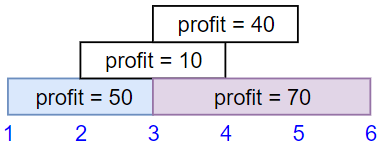
\includegraphics[width=7.7cm, height=3.1cm]{sample1.png}\begin{center}\textbf{Figure 1}\end{center}
\textbf{Input:}\\\\ startTime = [1,2,3,3]\\\\endTime = [3,4,5,6]\\\\profit = [50,10,40,70]\\\\Output: 120\\\\\textbf{Explanation:} The subset chosen is the first and fourth job. 
Time range [1-3]+[3-6] , we get profit of 120 = 50 + 70.

\paragraph{Dynamic Programming:}Dynamic Programming is mainly an optimization over plain recursion. Wherever we see a recursive solution that has repeated calls for same inputs, we can optimize it using Dynamic Programming. The idea is to simply store the results of subproblems, so that we do not have to re-compute them when needed later.\\\\This problem has both properties of Dynamic Programming, Optimal Substructure and Overlapping Subproblems. Like other Dynamic Programming Problems, we can solve this problem by making a table that stores solution of subproblems.\\\\This report further contains -\\\\II. Algorithm Design\\III. Pseudo Code\\IV. Algorithm Analysis\\V. Conclusion\\VI. References


\section*{II. ALGORITHM DESIGN}
\paragraph{Algorithmic Steps:}The algorithm is:\\\\1) Sort the jobs by non-decreasing finish times.\\\\2) For each i from 1 to n, determine the maximum value of the schedule from the subsequence of jobs[0..i]. Do this by comparing the inclusion of job[i] to the schedule to the exclusion of job[i] to the schedule, and then taking the max.\\\\3) To find the profit with inclusion of job[i]. we need to find the latest job that doesn’t conflict with job[i]. The idea is to use Binary Search to find the latest non-conflicting job.


\section*{III. PSEUDO CODE}
\lstset { %
    language=C++,
    backgroundcolor=\color{black!5},
    basicstyle=\footnotesize,
}

\begin{lstlisting}
FUNCTION findLatestJob(low, hi, v)
{
    
  pos <- -1
    
  while low <= hi 
  {
    int mid = (low + hi)/2
                
    if v[mid].first.second <= v[i].first.first 
    {                   
       pos <- mid
       low <- mid + 1
    }
    else{
       hi <- mid - 1
    }
  }
  
  return pos
}

FUNCTION findMaxProfit (v) {
    
    n <- v.size()
    
    dp : Vector of size n
        
    dp[0] <- v[0].second
        
    for i <- 1 to n
    {
        inc <- v[i].second;
        low <- 0
        hi  <- i - 1;
        
        pos <- findLatestJob(lo, hi, v)
            
        if pos != -1
        {
            inc += dp[pos]
        }
            
        exc <- dp[i-1]
        
        dp[i] <- max(inc,exc)
    }
    
    return dp[n-1]
}

FUNCTION main () {
    
    n 
    Input n
    
    startTime: Vector of size n
    endTime : Vector of size n
    profit : Vector of size n
    
    for i <- 0 to  n
        Input startTime
        Input endTime
        Input profit
    
    p : pair{startTime,endTime}
    v : Vector of pair{p,profit}
    
    sort v by end time
    
    print findMaxProfit (v) 

}
\end{lstlisting}
Code Link: \url{https://ideone.com/1QAHI3}
\section*{IV.ALGORITHM ANALYSIS}

Time Complexity - Time complexity is the number of operations an algorithm performs to complete its task (considering that each operation takes the same amount of time). The algorithm that performs the task in the smallest number of operations is considered the most efficient one in terms of the time complexity.\\\\Space Complexity - The space complexity of an algorithm is the amount of memory space required to solve an instance of the computational problem as a function of characteristics of the input. It is the memory required by an algorithm until it executes completely.\\\\Time Complexity – Sorting takes O(nlogn) time and also when we are iterating each element to find the maximum profit till each job and then using Binary Search based function to find the latest job (before current job) that doesn't conflict with current job which also takes O(nlogn) time so the overall time complexity is O(nlogn).\\\\Space Complexity – Since we are using dp array to store solutions of subproblems dp[i] stores the profit for jobs till arr[i] (including dp[i]). So the space complexity is O(n)\\\\
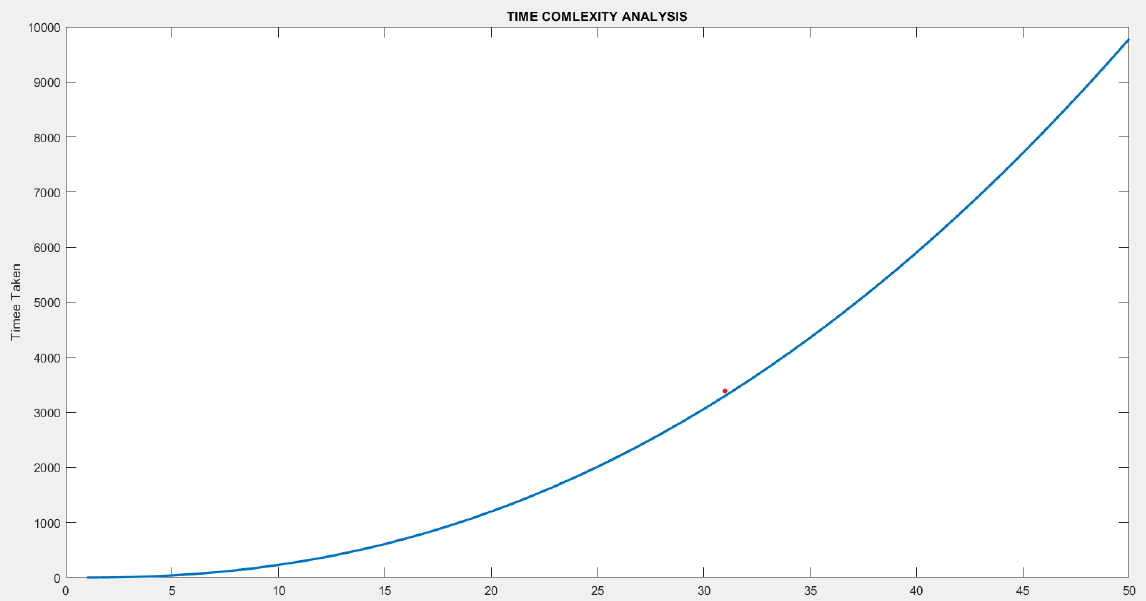
\includegraphics[width=\columnwidth, height=6cm]{Time Complexity.png}\begin{center}\textbf{Figure 2:} Time Complexity Graph\end{center}
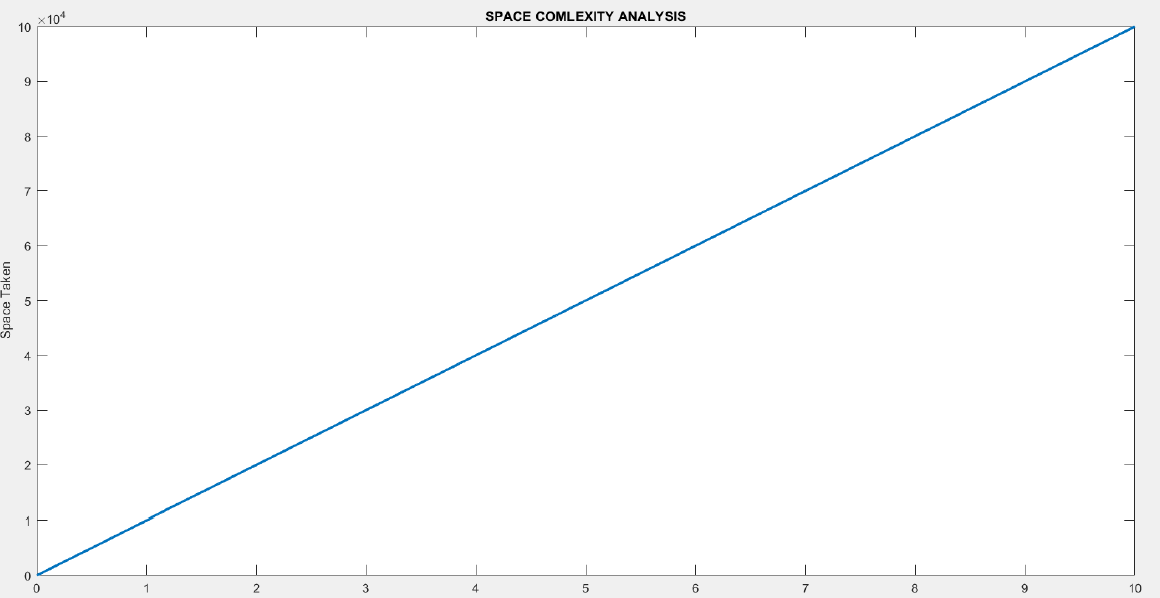
\includegraphics[width=\columnwidth, height=6cm]{Space Complexity.png}\begin{center}\textbf{Figure 3:} Space Complexity Graph\end{center}

\section*{V.CONCLUSION}

This problem could be solved efficiently in O(nlogn) time complexity and O(n) space complexity using dyanmic programming and binary search algorithm.

\section*{VI. REFERENCES}

\begin{enumerate}
\item Dynamic Programming\\
https://www.geeksforgeeks.org/dynamic-programming/
\item
https://www.geeksforgeeks.org/weighted-job-scheduling-log-n-time/
\item
https://leetcode.com/problems/maximum-profit-in-job-scheduling/
\item Time Complexity\\
https://www.freecodecamp.org/news/time-\\complexity-of-algorithms/
\item Space Complexity\\
https://en.wikipedia.org/wiki/Space\_complexity
\end{enumerate}
\end{multicols*}

	
\end{document}
